Wie im Kapitel Design bereits beschreiben, haben wir um die Website aufzulockern einige Animationen eingebaut. 
In folgendem Abschnitt wird erläutert, mit welchem Verfahren diese ausgewählt wurden, welche Technolgien verwendet wurden und die 
wie die Einbindung auf der Homepage funktioniert.

\section{Auswahl der Animationen und Grafiken} \label{sec:animationen:Aimationen}
\setauthor{Angerer Mona}

Als Grafiken wurde auf simple Darstellungen des Schulgebäudes der HTL Leonding aus verschiedenen Perspektiven gesetzt. 
Eine Abbildung aus der Vogelperspektive (Siehe Abbildung \ref{fig:impl:schule:oben}) ist implementiert in der Startanimation der Homepage, 
eine grafische Verwirklichung der Schule von vorne (Siehe Abbildung \ref{fig:impl:schule:vorne})
ist auf der Unterseite "Abteilungen" zu finden. Insbesondere die zuletzt erwähnte Grafik ist auch in Zukunft, nach Abschluss der Diplomarbeit
für vielseitige Zwecke einsetzbar und kann leicht modifiziert und angepasst werden.

Bei der Auswahl der eingebundenen Animationen wurde großer Wert auf die Benutzerfreundlichkeit und Navigation gelegt.
Deswegen wird beim Aufruf der neuen Homepage direkt mit einer etwa zwei-sekündigen Startanimation begonnen. Diese soll die 
Aufmerksamkeit der User erlangen und einen spannenden Start bieten. Sie startet mit dem HTL Leonding Logo und dem Schriftzug "HTL Leonding next level" und nachdem
das Logo von der linken Seite zur rechten Seite schwebt und der Schriftzug veschwindet verwandelt sich das Logo in eine Grafik des 
HTL Gebäudes aus der Vogelperspektive. Anschließend scrollen die wichtigsten News-Beiträge von rechts aus dem Gebäude. 
Auch wurde für jede Abteilung der HTL eine eigene kleine Animation gefertigt, die die jeweilige Fachriochtung repräsentiert.


\begin{figure}
   \begin{minipage}[b]{.4\linewidth} 
      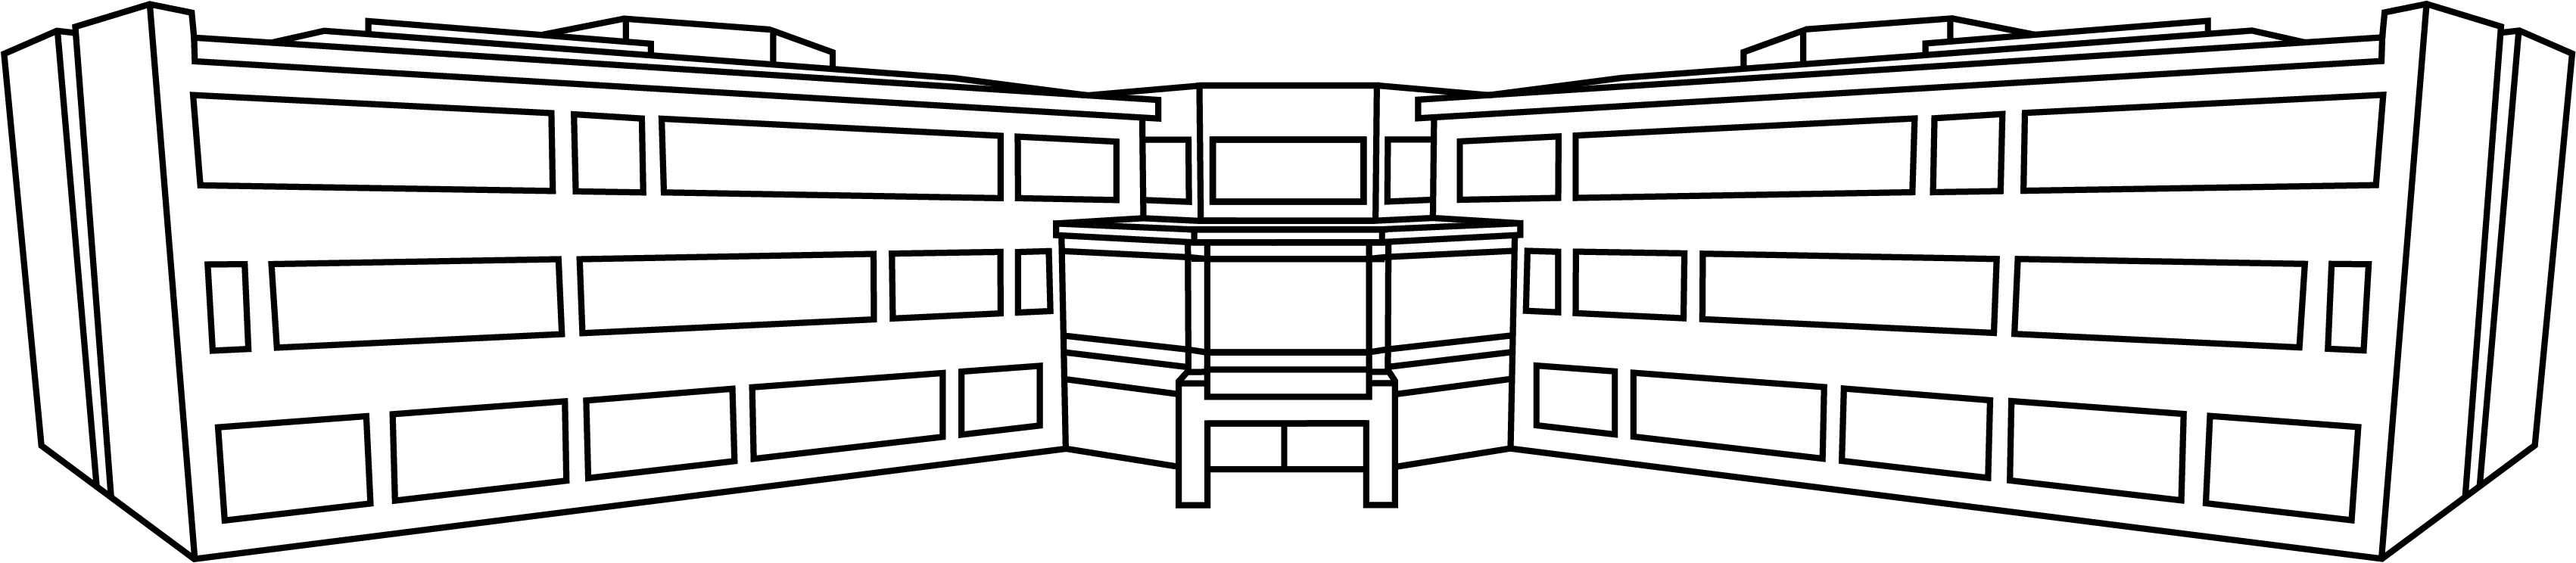
\includegraphics[width=\linewidth]{pics/schule vorne.png}
      \caption{SVG Schule von vorne}
      \label{fig:impl:schule:vorne}
   \end{minipage}
   \hspace{.05\linewidth}
   \begin{minipage}[b]{.4\linewidth}
      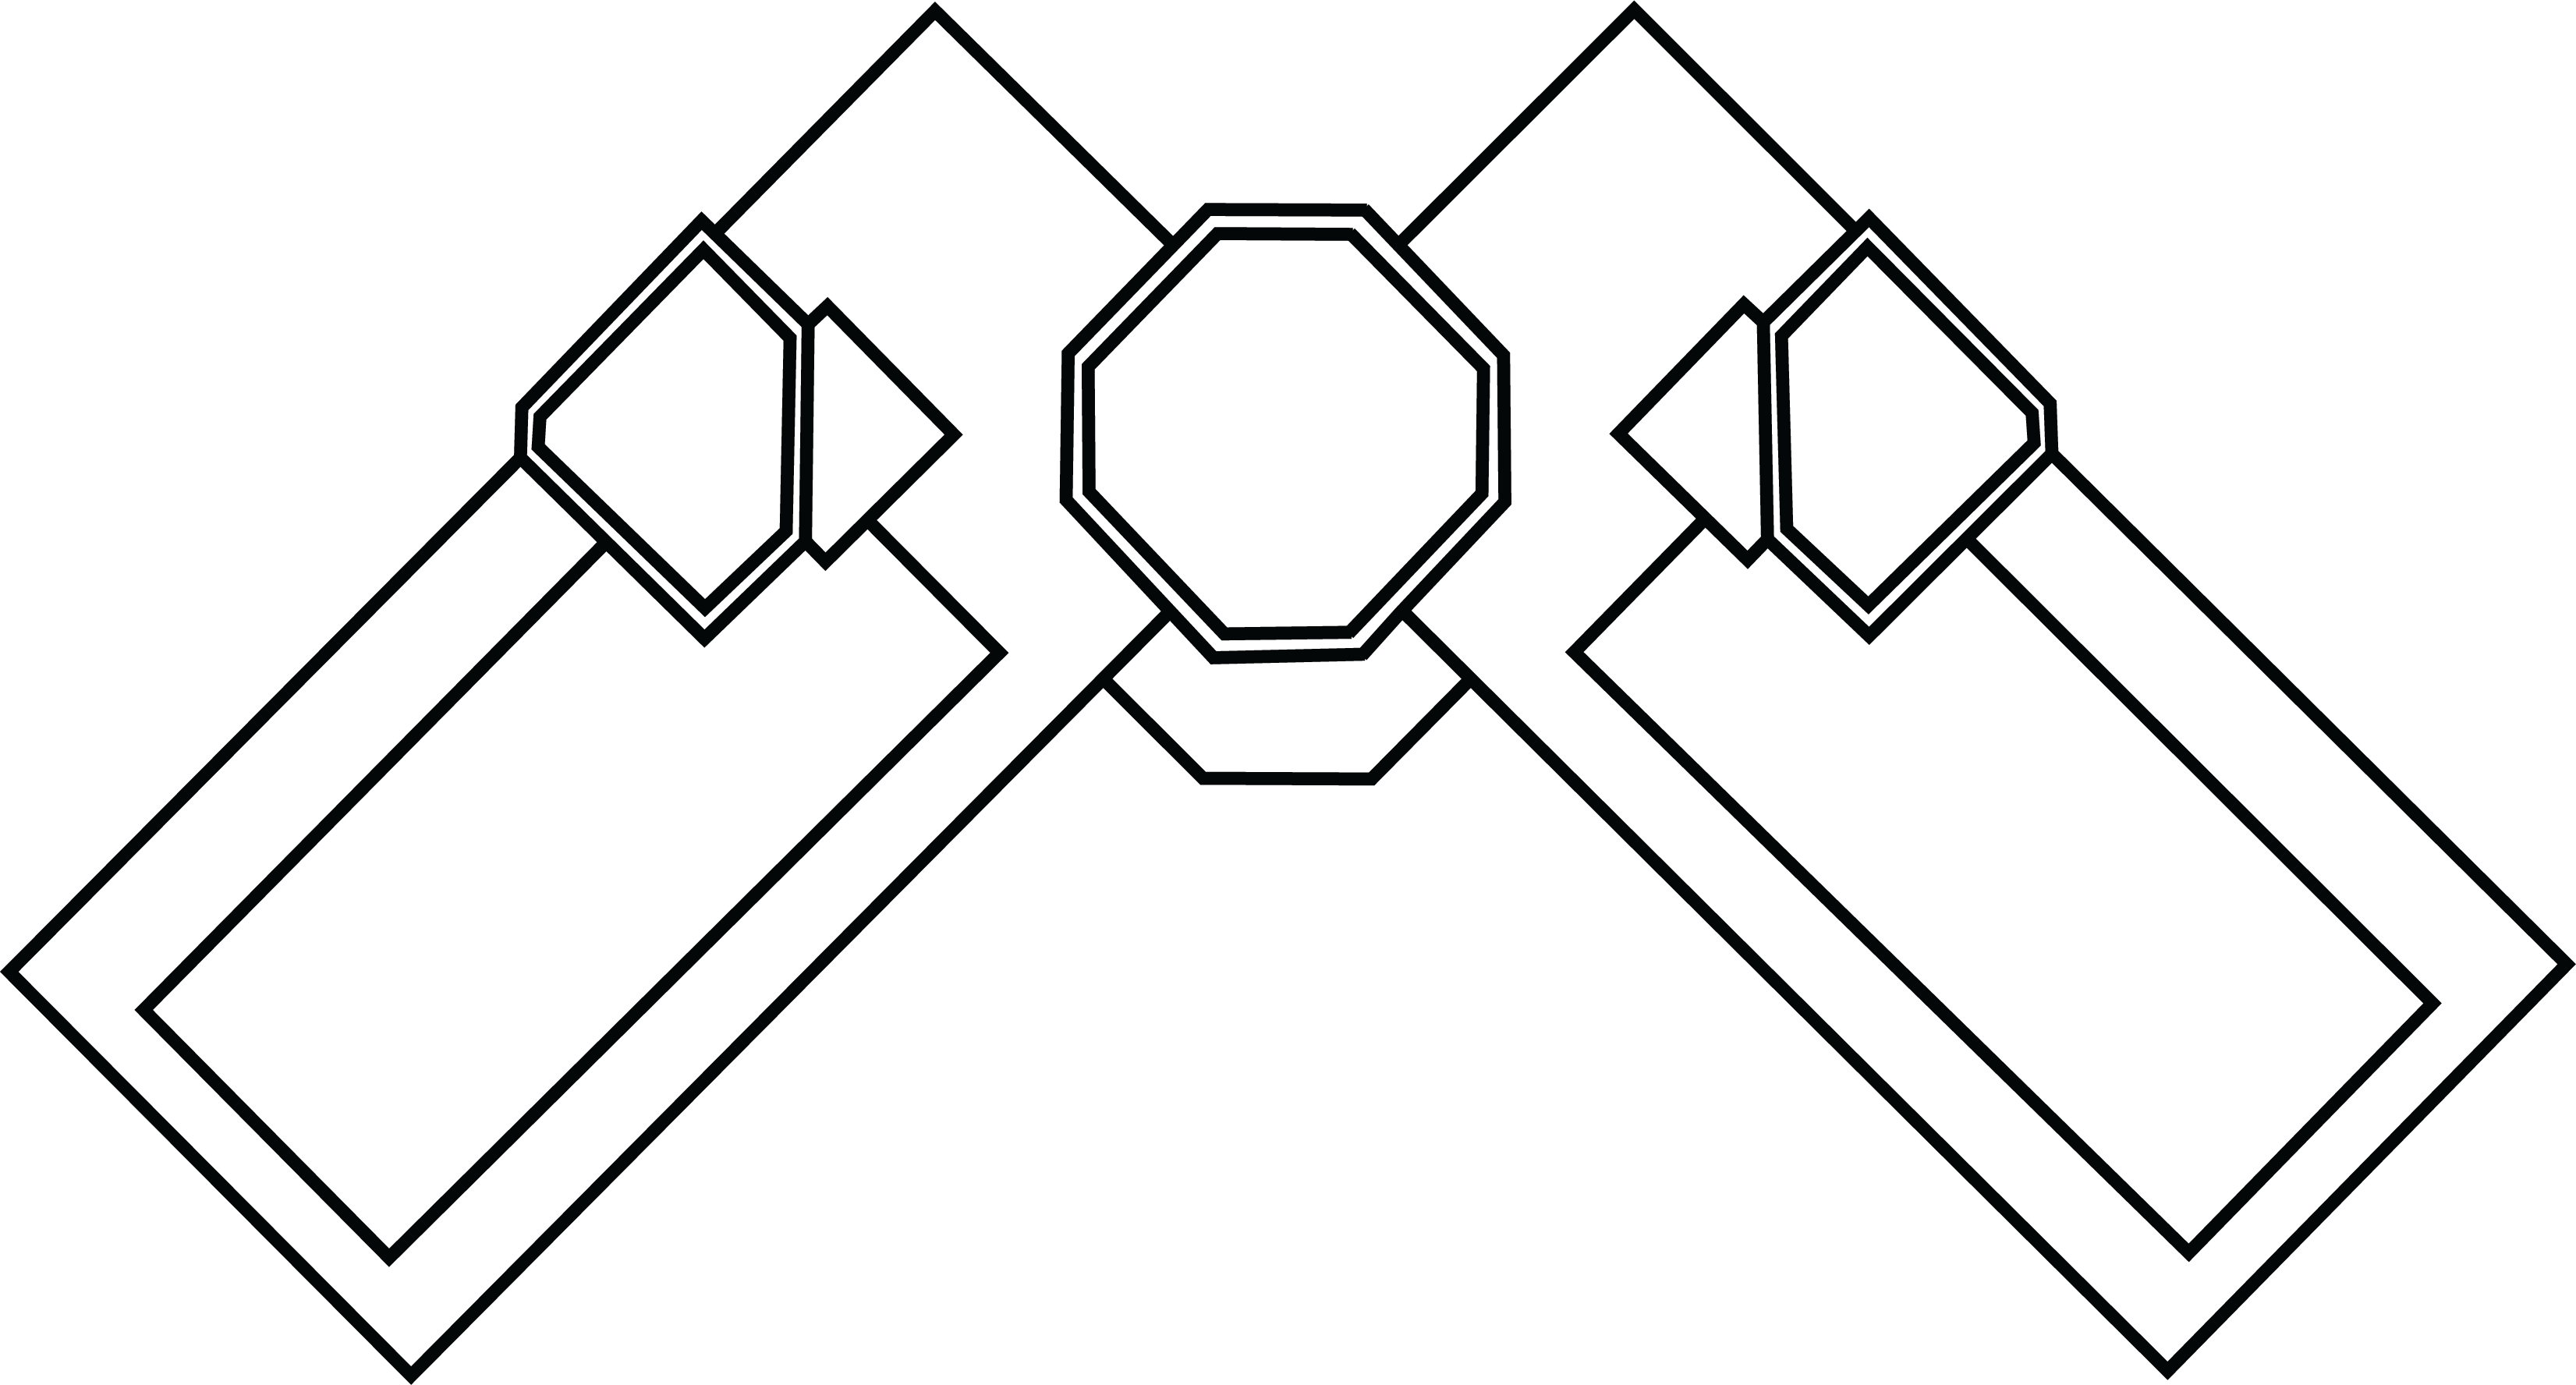
\includegraphics[width=\linewidth]{pics/schule.png}
      \caption{SVG Schule von oben}
      \label{fig:impl:schule:oben}
   \end{minipage}
\end{figure}


\section{Erstellung} \label{sec:animationen:Erstellen}
\setauthor{Angerer Mona}

Für jene Animationen, die nicht von Framer Motion umgesetzt werden, werden die Vektorgrafiken zuerst mittels Adobe Illustrator erstellt. Die Wahl der genutzten Programme zum Aufbereiten der Grafiken und Animationen fiel aus diversen Gründen
auf die Adobe Cloud. Einerseits sind die Anwendungen unter sich optimal kompartibel. Die Zusammenarbeit zwischen den Adobe-Programmen funktioniert 
einwandfrei und ermöglicht so einen optimierten Workflow. Die Vektorbasierte Arbeitsweise garantiert Grafiken ohne Qualitätsverlust bei jeder Skalierung. Auch bitet Illustrator die Möglichkeit, die erstellten Vektorgrafiken direkt als SVG zu exportieren, um anschließénd
in Adobe After Effects diese zu importieren und mit Animationstechniken zu veredeln. In After Effects können verschiedene Animationseffekte, 
Übergänge und Bewegungen hinzugefügt werden, um den Grafiken Leben einzuhauchen und sie dynamischer und ansprechender zu gestalten. 
Dieser Animationsprozess ermöglicht es, komplexe Bewegungen und Interaktionen zu erstellen, die die visuelle Darstellung der Grafiken 
erheblich verbessern.

Nach Abschluss der Animation in After Effects erfolgt der Export der animierten Grafiken im JSON-Format, welches von LottieFiles 
unterstützt wird. LottieFiles wird als Plugin in After Effects hinzugefügt und ist speziell für die Integration von animierten Grafiken in Web- und 
App-Designs entwickelt. Es ermöglicht die nahtlose Einbindung der animierten Grafiken in verschiedene Projekte und Plattformen, 
wobei die hohe Qualität und flüssige Darstellung der Animationen beibehalten wird. Durch die Verwendung von LottieFiles können die 
animierten Grafiken effizient in die Website integriert werden, ohne die Ladezeiten oder die Leistung der Website zu beeinträchtigen.


\section{Einbindung} \label{sec:animationen:Einbindung}
\setauthor{Angerer Mona}

\subsection{Framer Motion}
\setauthor{Mona Angerer}
Für die Umsetzung aller Animationen mit Ausnahme der SVG-Animationen auf der Website wurde das Animationsframework für React
Framer Motion ausgewählt. Es bietet eine leistungsstarke und flexible Lösung für 
die Erstellung von dynamischen und ansprechenden Animationen, die den HTML- und CSS-Code der Website betreffen.

Im Gegensatz zu herkömmlichen CSS-Animationen bietet Framer Motion ein breites Spektrum an fortschrittlichen 
Animationstechniken und -funktionen, die weit über einfache Transitions und Effekte hinausgehen. Eines der herausragenden 
Merkmale dieses Frameworks sind die Layout-Animationen, die es ermöglichen, komplexe seitenübergreifende Transformationen zu realisieren. 
Diese Layout-Animationen bieten die Möglichkeit, den Inhalt und die Struktur der Website dynamisch und ansprechend zu gestalten, 
wodurch ein flüssiges und nahtloses Benutzererlebnis geschaffen wird.

Darüber hinaus bietet Framer Motion spezialisierte Funktionen für Load- und Unload-Animationen. Diese sind darauf 
ausgerichtet, das Laden und Entladen des DOM (Document Object Model) zu animieren, um fließende und eindrucksvolle Seitenübergänge 
zu ermöglichen. Dies trägt maßgeblich zur Verbesserung der visuellen Darstellung und Benutzerfreundlichkeit der Website bei.

Die vielseitigen und erweiterten Funktionen von Framer Motion ermöglichen es, die Animationen und Interaktionen auf der 
Website gezielt und präzise zu steuern. Sie bieten eine hohe Flexibilität und Anpassungsfähigkeit, wodurch die individuellen 
 Animationseffekte leicht umgesetzt werden können.

 \subsection{Lottie}
\setauthor{Angerer Mona}
Als zentrales SVG-Animationsframework für die Implementierung der animierten SVG-Grafiken auf der Website wird Lottie verwendet. 
Dieses Framework bietet eine leistungsstarke Lösung für die Darstellung von komplexen und ansprechenden Animationen direkt im Webbrowser, 
ohne die Ladezeiten oder die Performance der Website negativ zu beeinflussen.

Nachdem Lottie als Plugin in After Effects hinzugefügt wird (zu finden in After Effects siehe Abbildung \ref{fig:impl:plugin:lottie}), können im Exportprozess aus Adobe After Effects die Animationen speziell als Lottie JSON 
exportiert, wodurch eine nahtlose und fehlerfreie Kompatibilität zwischen den beiden Programmen garantiert wird. Die gewonnenen JSON-Files 
können anschließend problemlos in die 
Website eingebunden werden.

\begin{figure}
   \begin{minipage}[b]{.4\linewidth} 
      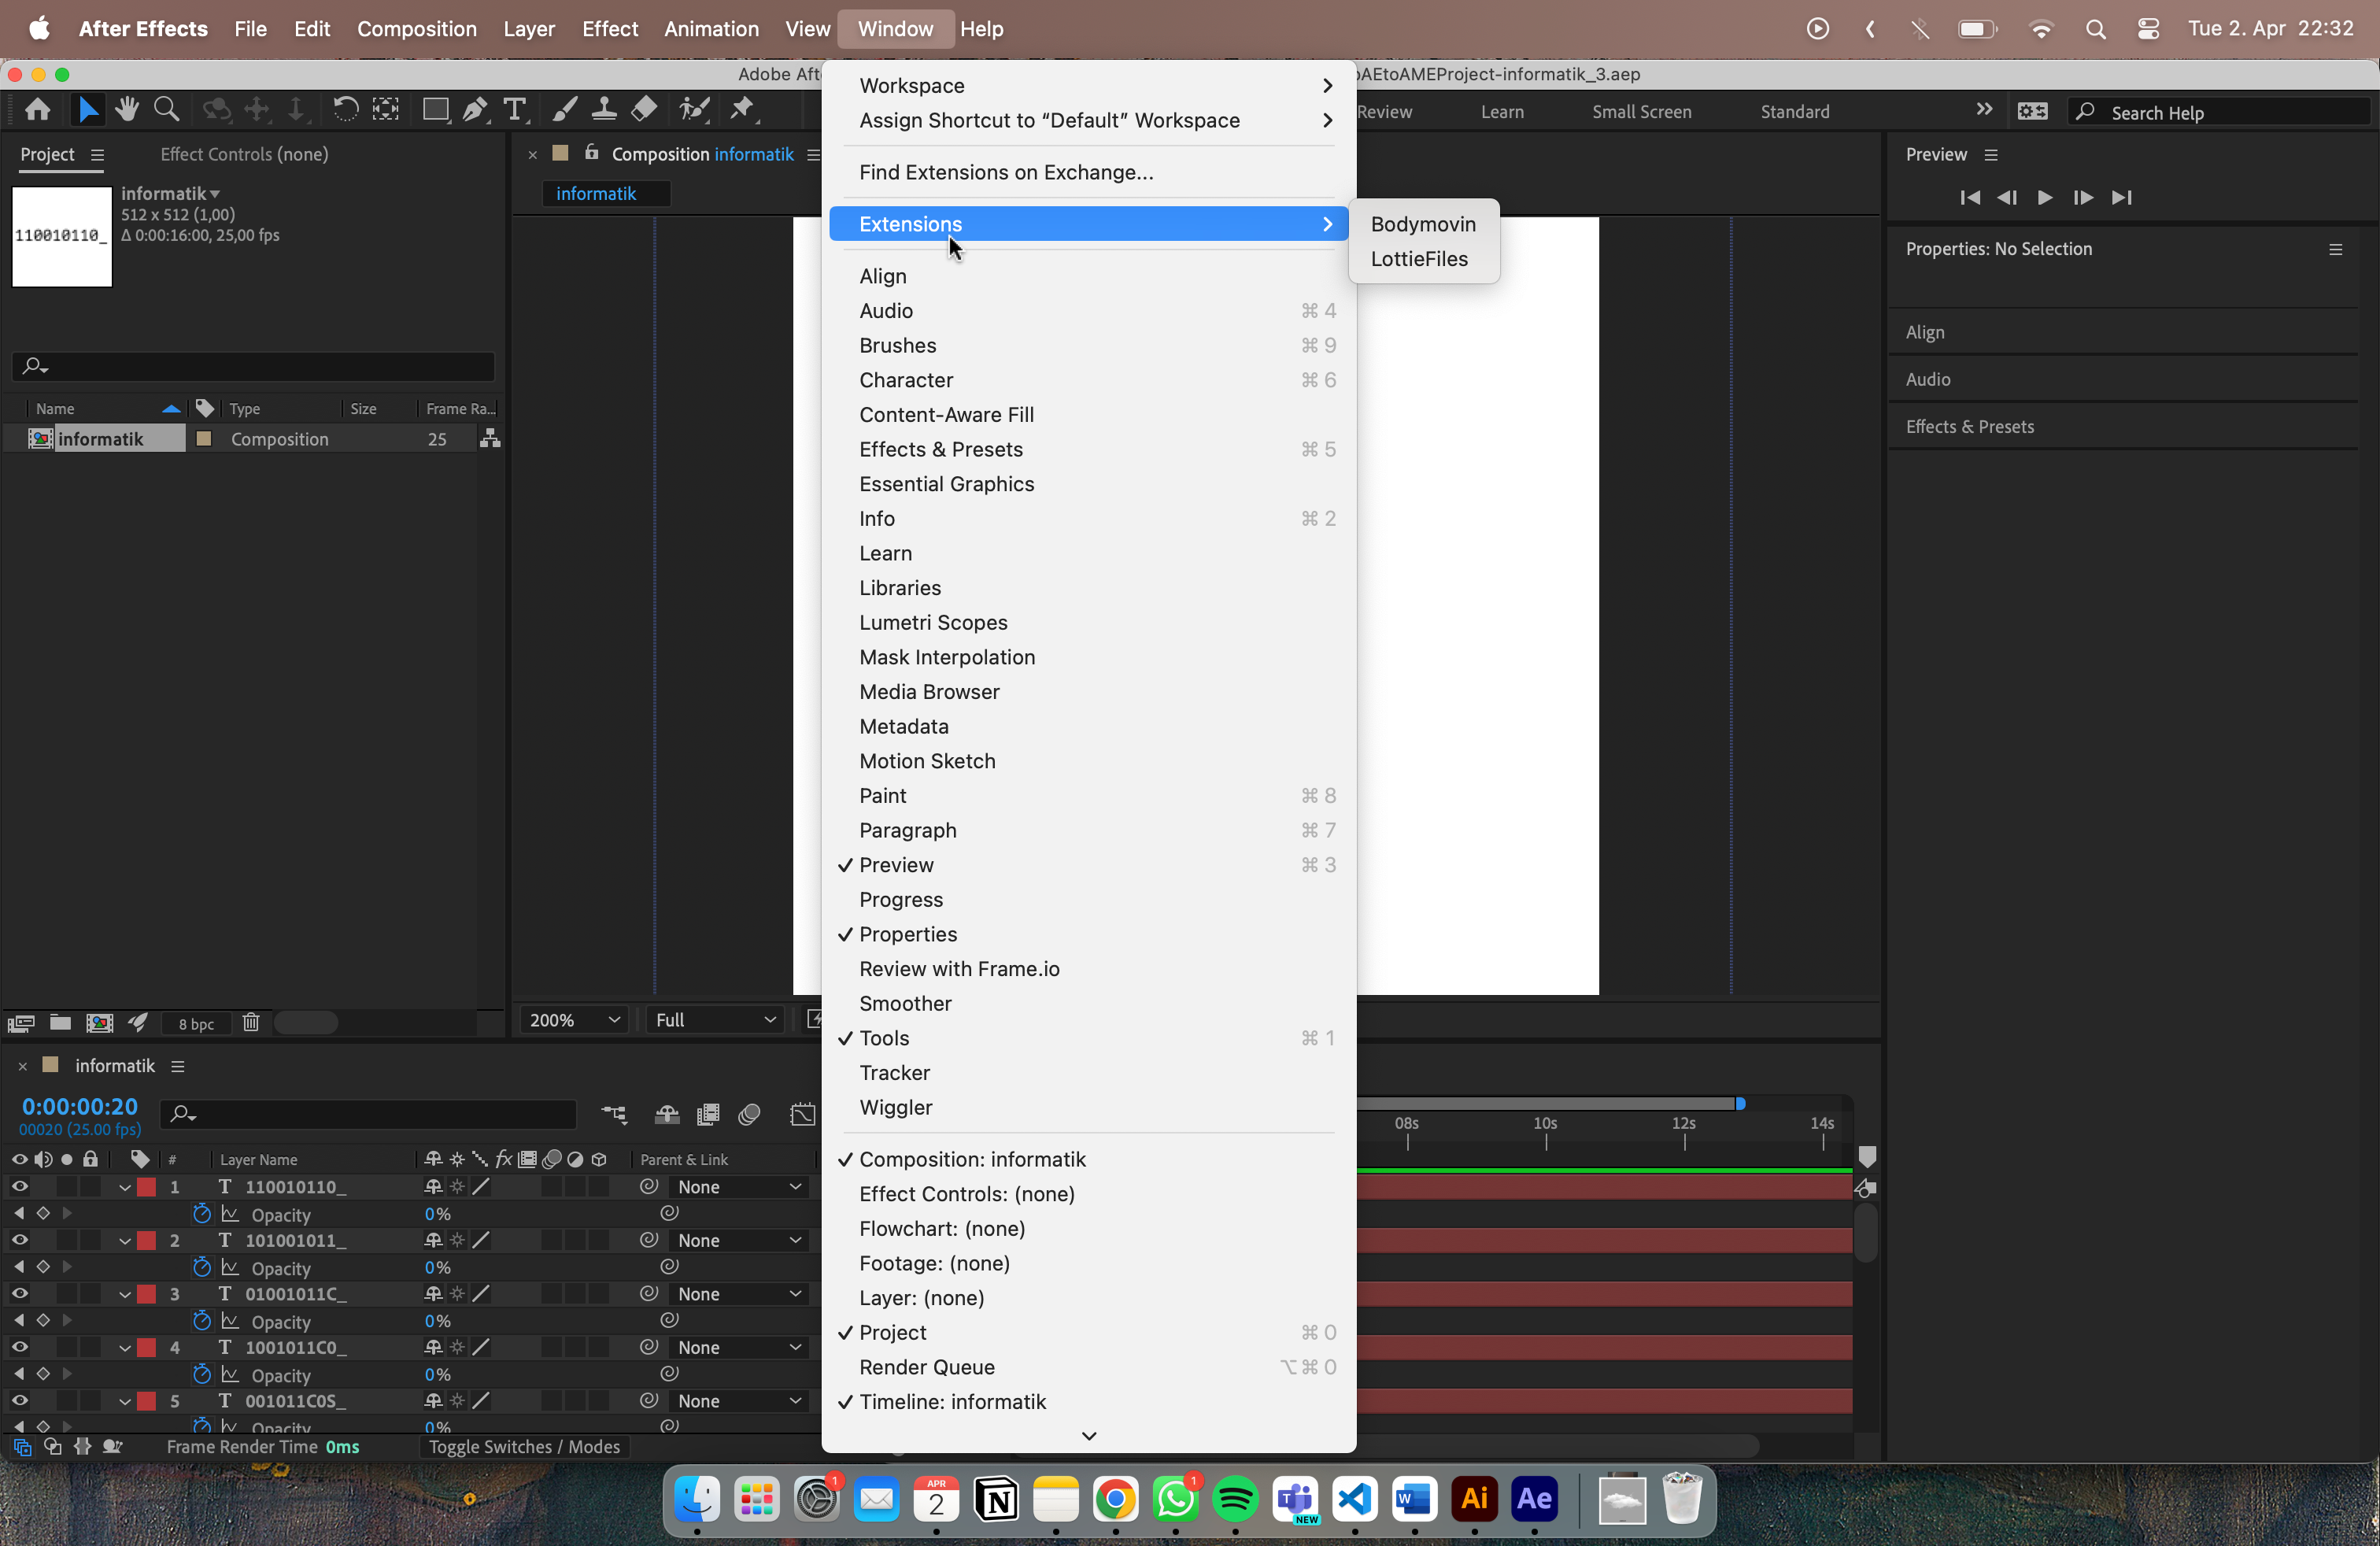
\includegraphics[width=\linewidth]{pics/plugin lottie.png}
      \caption{Lottie als Plugin in After Effects}
      \label{fig:impl:plugin:lottie}
   \end{minipage}
\end{figure}

Nach dem Export erfolgt die Implementierung der animierten Grafiken im Code durch die Einbindung dieser JSON-Dateien 
in den Lottie Player. Der Lottie Player ist ein spezialisiertes JavaScript-Plugin, das die Darstellung der Lottie JSON-Dateien im 
Webbrowser steuert. Durch diese Kombination werden alle übrigen Animationen, die nicht durch Framer Motion oder andere Technologien 
gesteuert werden können, effizient und zuverlässig durch Lottie gesteuert.

Beschreibene Vorgehensweise bietet den Vorteil, dass komplexe und detailreiche Animationen, die mit Adobe After Effects erstellt wurden, 
direkt und ohne Qualitätsverlust auf der Website dargestellt werden können. Die Verwendung von Lottie bietet eine höhere 
Flexibilität und Anpassungsfähigkeit der Animationen, da sie leicht aktualisiert oder modifiziert werden können, ohne den gesamten Code 
oder die Website neu zu laden.


\section{Schwierigkeiten} \label{sec:animationen:Schwierigkeiten}
\setauthor{Angerer Mona}

Als eine der größten Schwierigkeiten im Punkt Animationen und Grafik bot die Unstimmigkeit und Vielzahl der Ideen. Viele Male wurden Animationen
erstellt, die es im Endeffekt doch nicht auf die Endversion der Homepage geschafft haben, da sich neue und bessere Ideen boten. Dies stellte sich 
als große zeitliche Hürde da und forderte viele Arbeitsstunden.
Auch bereitete der Export der Animationen und die anschließende Einbindung auf der Website einige Schwierigkeiten. 
Da die Ursprungsidee, die Animationen als Videodatein einzubinden aufrgund resultierender hoher Ladezeiten und eingeschreänkter Interaktivität
schnell verworfen wurde, lag die Lösung, JSON-Animationen zu benutzen, nahe.
Es gab zwischenzeitliche Probleme, als versucht wurde die Animaitonen aus After Effects mittels Bodymovin (ein Plugin für Adobe After Effects, das es ermöglicht, 
Animationen aus After Effects-Projekten in das JSON-Format zu exportieren) zu rendern, da einige Bilddatein von dem Plugin nicht richtig interpretiert wurden.

